\documentclass[12pt,a4paper]{article}
\usepackage[portuges]{babel}
\usepackage[utf8]{inputenc}
\usepackage[T1]{fontenc}
\usepackage{amsmath}
\usepackage{amsfonts}
\usepackage{amssymb}
\usepackage{pgfplots}
\usepackage{filecontents}
\usepackage{cite}
\usepackage{subfigure}
\usepackage{tikz}
\usepackage{caption}
\usepackage{graphicx}
\usepackage{float}
\usepackage[lined,boxed,commentsnumbered]{algorithm2e}
\usepackage{rotating}

%%%%%%Information of the paper
\pdfinfo{
/Title (EP4 - Planejamento Probabilístico)
/Author (Diego Araujo, Viviane Bonadia, Ignasi Andres)
}

%%%%%%%%Title
\title{MAC5788 - Relatório EP4: Planejamento Probabilístico}
\author{Viviane Bonadia NUSP 9167607, Diego Ara\'{u}jo NUSP 7157092, \\ Ignasi Andr\'{e}s NUSP 8193481\\
Universidade de S\~{a}o Paulo\\
S\~{a}o Paulo, Brazil\\ \{vbonadia, diegoamc, ignasi\} @ime.usp.br}

\begin{document}
\maketitle

\section{Introdução}


O planejamento consiste na elaboração de um plano de ação, ou seja um conjunto de ações, para atingir um determinado objetivo \cite{russell1995artificial}. No planejamento probabilístico os efeitos das ações possuem uma incerteza, quando uma ação é executada em um determinado estado, não existe uma certeza sobre qual será o próximo estado. O que sabemos é uma distribuição de probabilidade dos estados alcançáveis.
Implementamos e realizamos diversos experimentos com quatro algoritmos para encontrar uma política em problemas de planejamento probabilístico: ILAO$^*$, RTDP, LRTDP,  e VI que serão melhor explicados ao longo deste relatório. Este trabalho está organizado da seguinte maneira: na seção \ref{planejamento} descrevemos mais detalhadamente Planejamento Probabilístico, na seção \ref{algoritmos} descrevemos cada um dos algoritmos implementados, na seção \ref{implementacao} descrevemos alguns detalhes da nossa implementação, na seção \ref{experimentos} apresentamos os experimentos realizados bem como os resultados obtidos e, por fim, na seção \ref{conclusao} expomos as conclusões obtidas com este trabalho.


%%%%%%%%%%%%%%%%%%%%%%%%%%%%%%%%%%%%%%%%%%%%%%%%%%%%%%
\section{Planejamento probabilístico} \label{planejamento}


Em problemas de planejamento clássico, executar uma ação em um determinado estado leva o agente para um outro único estado. No planejamento probabilíıstico, a realização de uma ação pode levar o agente à diferentes estados. Ou seja, não é possível saber com certeza qual será o próximo estado do agente após escolher uma determinada ação. O que conhecemos, em problemas desse tipo, são as probabilidades que o agente tem de, dado um estado  $s$ ele alcançar um estado $s'$ ao escolher uma determinada ação.

A solução para problemas de planejamento probabilístico é uma política $\pi$. Uma política mapeia os estados do problema em ações de forma a otimizar a escolha das ações segundo algum critério (por exemplo custo ou recompensa).

Podemos resolver problemas de planejamento probabilístico usando Processo de Decisão Markoviano (MDP) para representá-los. Um MDP pode ser definido como uma tupla $\langle S, A, R, P, \gamma \rangle$ onde:

\begin{itemize}
  \item $S$ é o conjunto finito de estados
  \item $A$ é o conjunto finito de ações
  \item $R$ é o modelo recompensa associado a cada par $\langle$estado, 
ação$\rangle$
  \item $P$ é o modelo de transição probabilístico. $P(s'|s,a)$ é a probabilidade de um agente que está no estado $s \in S$ ir para o estado $s' \in S$ ao executar a ação $a \in A$
  \item $\gamma$ é o fator de desconto ($0 \leq \gamma < 1$)
\end{itemize}


Um MDP poder ser de horizonte finito ou infinito. Neste segundo caso, o agente não altera  a forma de agir com o passar do tempo e seu objetivo é encontrar uma política ótima que maximiza a recompensa descontada num horizonte infinito.

A função valor ótima (V$^*$) é a função que está associada a qualquer política ótima e deve satisfazer a seguinte equação:

\begin{equation}\label{bellman}
V^*(a) = \max_{a\in A(s)}\{R(s,a) + \gamma \sum\limits_{s'\in S} P(s'|s, a) V^*(s')\}
\end{equation}

Existem diversos algoritmos que resolvem este tipo de problema. Os algoritmos implementados neste trabalho são alguns exemplos propostos para problemas de planejamento probabilístico.

%Podemos definir a função valor do estado como a recompensa esperada a partir do estado $s$ como $V(s)$, e a função $Q(s,a)$ como a recompensa esperada a partir do estado $s$ executando a ação $a$.







%%%%%%%%%%%%%%%%%%%%%%%%%%%%%%%%%%%%%%%%%%%%%%%%%%%%%%
\section{Algoritmos}\label{algoritmos}

\subsection{VI}\label{vi}
O Algoritmo Iteração de Valor (VI) \cite{Bellman57} garante encontrar uma política ótima usando programação dinâmica. 

Na primeira iteração o algoritmo inicia V(s) com valores arbitrários e, a cada iteração, atualiza V(s) para todos os estados segundo a Equação \ref{bellman}. O algoritmo termina quando o valor residual é menor que $\varepsilon$.

O valor residual é a diferença entre os valores $V(s)_i$ (calculados na iteração atual) e $V(s)_{i-1}$ (calculados na última iteração). $\varepsilon$ é um valor muito pequeno, definido no algoritmo. Em nossa implementação usamos $\varepsilon=10^{-7}$.

A cada iteração, este algoritmo atualiza todos os estados e, como o espaço de estados pode ter tamanho exponencial, problemas mais complexos tornam-se inviáveis de resolver.

Em razão da atualização de todos os estados a cada iteração, o VI é chamado de solução síncrona.

\subsection{RTDP}\label{rtdp}

O algoritmo RTDP (\textit{Real-Time Dynamic Programming}) \cite{barto95} diferente do algoritmo VI, não garante como solução uma política ótima. Porém, RTDP encontra valor ótimo para todos os estados relevantes. Estados relevantes são aqueles alcançáveis a partir do conjunto de estados inicial segundo uma política ótima.

Assim como o algoritmo VI, ele também inicia $V(s)$ com valores arbitrários porém, a cada iteração o algoritmo recalcula o valor de $V(S)$ apenas para o estado atual usando a Equação \ref{bellman}, por esse motivo RTDP é um exemplo de algoritmo de programação dinâmica assíncrona.

Após a etapa de inicialização, o RTDP executa várias simulações (\textit{trials}). A cada simulação um estado do conjunto de estados inicial é escolhido aleatoriamente. Para obter o próximo estado, o algoritmo sorteia o próximo estado a partir da função de transição $P(.|s, a)$. RTDP termina um trial se encontrar um estado meta ou quando uma profundidade limitada é alcançada.

O RTDP não tem condição de parada. Portanto, em nossos experimentos, consideramos um \textit{timeout} de 1 minuto. Esse valor foi escolhido baseado no tempo de execução do algoritmo LRTP, explicado a seguir.


\subsection{LRTDP}\label{lrtdp}


O algoritmo LRTDP (\textit{Labeled Real-Time Dynamic Programming}) \cite{Bonet03labeledrtdp}, baseia-se no algoritmo RTDP. Ele introduz uma heurística ao algoritmo RTDP e, diferente deste, devolve uma política parcialmente ótima. A política é chamada de parcialmente ótima por devolver uma política ótima apenas para os estados relevantes partindo do estado inicial estado inicial até o estado meta.

Enquanto no algoritmo RTPD, quanto maior a probabilidade de um estado $s$ ser alcançado mais vezes seu valor função $V(s)$ será atualizado, no LRTDP os estados que já convergiram são rotulados. A cada novo \textit{trial} o algoritmo irá priorizar a atualização dos estados que ainda não convergiram (e não apenas os caminhos com maior probabilidade) aumentando a velocidade de convergência do algoritmo.

O algoritmo termina quando o estado inicial converge com valor residual menor que um determinado $\varepsilon$. Neste trabalho, consideramos $\varepsilon=10^{-7}$.

É importante notar que tanto o LRTDP quanto o RTDP tem comportamento \textit{anytime}. Isso significa que eles podem produzir uma boa política rapidamente e melhorá-la com o tempo.

\subsection{iLAO$^*$}\label{ilao}
%copy paste Ignasi com pequenas alterações

O algoritmo ILAO$^*$ (\textit{Improved LAO$^*$}) \cite{ilao}, assim como RTDP e 
LRTP, utiliza programação dinâmica na atualização dos estados.

O princípio deste algoritmo também consiste em criar \textit{trials} ou caminhos entre o estado inicial e um estado meta.

Se chegarmos a um estado meta, o algoritmo executa o algoritmo Value Iteration entre os estados do caminho. 

Se o algoritmo encontrar um estado novo que não foi adicionado no caminho, ou algum estado que ainda não convergiu, ele realiza um novo \textit{trial} e assim sucessivamente até que todos os estados no caminho estejam convergidos, e nenhum caminho novo seja encontrado.

O algoritmo $LAO^*$ original executa o algoritmo VI sempre que adiciona um novo estado no caminho. Esta versão do algoritmo é menos eficiente. Por isso, os autores propuseram uma versão na qual a etapa de execução do VI somente é executada quando um caminho é descoberto.

Uma das vantagens deste algoritmo a respeito da família RTDP é que ele analisa não somente os estados com maior probabilidade de serem alcançados, mas todos os estados que podem ser alcançados a partir de uma mesma ação não determinística. Isso pode acelerar o tempo de convergência do algoritmo, uma vez que, a cada iteração, ele atualiza um maior número de estados.


%%%%%%%%%%%%%%%%%%%%%%%%%%%%%%%%%%%%%%%%%%%%%%%%%%%%%%
\section{Implementação}\label{implementacao}

Nesta seção, apresentaremos como executar o programa e alguns detalhes de implementação, ressaltando decisões importantes que tomamos durante o desenvolvimento.

\subsection{Como executar o programa?}\label{implementacao:execucao}

O projeto foi implementado usando a linguagem de programação Ruby. Portanto, para rodá-lo é preciso ter o Ruby (versão acima da 1.9.3) instalado no computador. 

Na raiz do projeto (diretório $probabilistic\_planning$) execute o seguinte comando:

\begin{center}
{ruby probabilistic\_planning.rb <domínio> <algoritmo>}
\end{center}

\begin{itemize}
\item <domínio> é o nome do domínio que será usado, os parâmetros aceitos são: \textbf{tireworld} ou \textbf{navigation\_problem}

\item <algoritmo> é o nome do algoritmo utilizado para gerar a política, os parâmetros aceitos são: \textbf{ILAO}, \textbf{LRTDP}, \textbf{RTDP} ou \textbf{VI}.
\end{itemize}

Um exemplo do comando é dado a seguir:

\begin{center}
{ruby probabilistic\_planning.rb tireworld ILAO}
\end{center}

Esse comando rodará o EP para todos os problemas do domónio Tireworld disponíveis no diretório $problems/tireworld$. Após a execução, os resultados estarão disponíveis no diretório $results/tireworld$. É preciso criar este diretório manualmente para que os resultados sejam corretamente armazenados.



\subsection{Detalhes do código}\label{implementacao:detalhes}
Cada uma das classes e seus principais detalhes de implementação são explicados a seguir.

\begin{itemize}
    \item \textbf{requirements.rb}: classe que inclui todas as dependências do programa.
    \item \textbf{parser.rb}: classe que lê a descrição dos problemas e a mapeia em objetos do domínio, como estados e ações.
    \item \textbf{probabilistic\_planning.rb}: arquivo que roda o programa. São recebidos dois parâmetros, os nomes do domínio e do algoritmo que será utilizado para resolver os problemas do domínio. É assumido que existe um diretório \textit{results} criado, com dois subdiretórios, \textit{tireworld} e \textit{navigation\_problem} (nome domínios suportados). O resultado dos algoritmos para cada problema em específico será armazenado dentro do diretório do seu respectivo domínio. Todos os problemas do domínio escolhido serão executados. A descrição deles pode ser encontrada nos subdiretórios do diretório \textit{problems}.
    \item \textbf{domain/state.rb}: abstração dos estados. Possui atributos, como \textit{stacked}, \textit{visited} e \textit{greedy\_action} que auxiliam na elaboração da saída e cálculo de métricas para cada algoritmo.
    \item \textbf{domain/action.rb}: abstração das ações. O destino de cada ação é tratado como uma matriz, na qual cada linha representa um destino, a primeira coluna é a probabilidade e a segunda é o estado final.
    \item \textbf{domain/problem\_definition.rb}: abstração do problema. É usada para fazer o cadastro dos estados e suas respectivas ações. Guarda informações gerais do problema, como estado inicial, meta e fator de desconto. Ordena os destinos de cada ação por ordem decrescente de probabilidade.
    \item \textbf{algorithms/procedures.rb}: módulo que possui funções comuns dos algoritmos implementados. É importante notar que levamos em consideração o fator de desconto do problema e a recompensa da ação do cálculo do \textit{qValue}. A ação gulosa escolhida é aquela que possui maior \textit{qValue}. Usamos uma distribuição de probabilidade uniforme para decidir qual o próximo estado escolhido.
    \item \textbf{algorithms/vi.rb}: implementação do algoritmo Iteração de Valor. A condição de parada é que todos os estados tenham convergido, ou seja, que o valor do residual de cada um deles seja menor que $\varepsilon=10^{-7}$.
    \item \textbf{algorithms/rtdp.rb}: implementação do algoritmo RTDP. Apesar de explorar apenas os estados relevantes, não apresenta condição de parada. Portanto, aqui definimos um \textit{timeout} de 1 minuto para o algoritmo, baseado no tempo de execução do LRTDP. Resolvemos os \textit{dead ends} com um contador que verifica se a simulação (\textit{trial}) permanece no mesmo estado por mais de 30 vezes seguidas. Se isso acontecer, o \textit{trial} é interrompido.
    \item \textbf{algorithms/lrtdp.rb}: implementação do LRTDP. Esse algoritmo é uma melhora do RTDP ao rotular os estados já resolvidos. O algoritmo para quando o estado inicial é resolvido. Para determinar se um estado está resolvido ou não, verificamos se seu residual é menor que $\varepsilon=10^{-7}$. Resolvemos os \textit{dead ends} com um contador que verifica se a simulação (\textit{trial}) permanece no mesmo estado por mais de 30 vezes seguidas. Se isso acontecer, o \textit{trial} é interrompido.
    \item \textbf{algorithms/ilao.rb}: implementação do algoritmo iLAO*. O critério de parada desse algoritmo é a convergência dos estados relevantes. Um estado convergiu se seu residual é menor que $\varepsilon=10^{-7}$. Neste algoritmo resolvemos os \textit{dead ends} colocando os estados visitados em uma pilha. Se o estado atual já está na pilha, o algoritmo simplesmente termina o \textit{trial} e vai para o próximo.
\end{itemize}
%TODO falar o que é política não própria -> deadends
% Explicar o que fizemos para contornar os dead ends
% Precisa explicad cada uma das classes? (acho que não...talve so citar o que vaca arquivo tem implementado)
% Falar do fator de desconto?




%%%%%%%%%%%%%%%%%%%%%%%%%%%%%%%%%%%%%%%%%%%%%%%%%%%%%%
%Links para os resultados:
% https://docs.google.com/spreadsheets/d/1acyyi2MiCz10SoIB_6LjU7MmwAc5QRt3f3zG1oizbpE/edit?usp=sharing

%Brucutu:
% http://www.ime.usp.br/~vbonadia/plan_probabilistic/results/

\section{Experimentos e Resultados}\label{experimentos}

Rodamos os algoritmos implementados em dois domínios: Navigation e TireWorld, descritos nas seções \ref{navigation} e \ref{tireworld} respectivamente. Durante a execução do algoritmo, extraímos diversas métricas do problema dentre elas: tempo de execução do algoritmo, número de estados expandidos, estados visitados e número de \textit{trials}. Usamos essas métricas para analisar o desempenho de cada um dos algoritmos dos experimentos realizados.


\subsection{Domínio Navigation}\label{navigation}

Neste domínio, temos uma grade e um robô deve ir de uma localização origem (estado inicial) da grade para uma localização destino (estado meta).
O robô pode se movimentar para o norte, sul, leste ou oeste ou ainda escolher permanecer no mesmo lugar em que se encontra (ação noop).

Para cada estado em que o robô se encontra, ao executar uma determinada ação, pode existir uma probabilidade $p > 0$ do robô quebrar e se tornar impossível dele continuar sua trajetória e consequentemente alcançar a meta.

Para todo estado alcançado que não seja um estado meta, o robô recebe uma penalização.

A Figura \ref{fig:navigation} mostra um exemplo de uma instância do problema para este domínio. Na figura, as regiões em destaque (cor cinza) representa posições na grade onde, ao executar a ação que move o robô para o sul, existe uma probabilidade do robô quebrar. A posição onde está a bandeira, representa o estado meta.

\begin{figure}[H]%[htb]
  \centering
  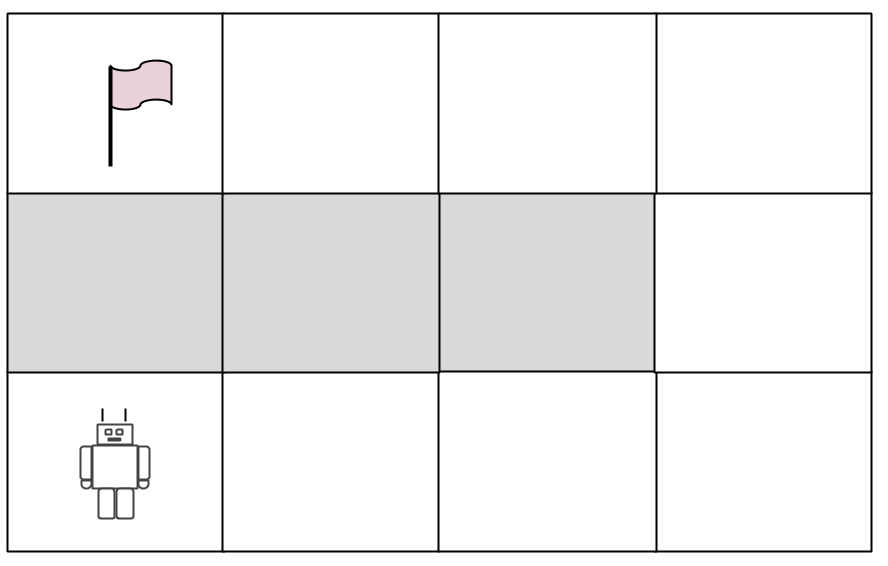
\includegraphics[width=8cm]{figures/navigation2.png}
  \caption{Exemplo de uma instância de problema do Domínio Navigation}
  \scriptsize
  Posições em destaque (cinza) representam posições da grade em que, ao executar a ação de mover para o sul e alcançar alguma dessas posições, existe uma probabilidade do robô quebrar.
  \label{fig:navigation}
\end{figure}

\subsubsection{Experimentos com o Domínio Navigation}
\label{experimentosNavigation}

Rodamos os algoritmos para doze diferentes problemas desse domínio. Cada problema variou o número de posições possíveis na grade, diferentes estados com probabilidade do robô quebrar, posição inicial e final. %A Tabela \ref{tab:navigation} apresenta resumidamente as características de cada um dos problemas.

%\begin{table}[H]

%TODO colar a tabela aqui
% nome do problema
% Quantidade de posições da grade
% quantidade de estados ruins para cada ação {norte, sul, leste, oeste}

\caption{Características dos problemas utilizados para o domínio Navigation}
\label{tab:navigation}
\end{table}


\subsubsection{Resultados para o Domínio Navigation}\label{resulsNavigation}
A Figura \ref{fig:timeNav} exibe o tempo de execução de cada um dos algoritmos. Ao observarmos ela, é possível perceber que nos domínios menores, ou seja, domínios onde o espaço de estados possíveis é menor (por exemplo Nav-01, Nav-02, Nav-03 e Nav-04) o algoritmo $LRTDP$ converge mais rapidamente quando comparado ao $ILAO$. Porém, a partir do momento em lidamos com problemas maiores, o $ILAO$ passa a apresentar resultados melhores. 

Como o $RTDP$ não possui uma condição de parada, nos experimentos definimos o \textit{timeout} de execução em 1 minuto. Isso explica porque seus resultados estão muito acima dos demais algoritmos.

Os demais algoritmos ($ILAO$, $LRTDP$ e $VI$) que tem como critério de parada a convergência dos estados, o $VI$ foi o que apresentou um desempenho pior. Ou seja, levou um tempo maior para convergir.

%Grafico para time - Navigation
\begin{figure}[H]
\centering
\begin{tikzpicture}
  \begin{axis}[
      xtick=data, 
      xticklabels from table={plots/timeNav.dat}{Problema},
      xticklabel style={rotate=90},
      axis lines=left,
      xlabel={Problemas Navigation},
      xlabel style={at={(0.5,-0.15)}},
      ylabel={Tempo de Execução em milissegundos},
      enlarge x limits={abs={0.0001*\pgfplotbarwidth}},
      legend style={at={(0.25,0.4)},anchor=north,legend columns=2},
      height=9cm, width=12cm,
      ymode=log]

      \addplot table [x expr=\coordindex,y=ILAO]{plots/timeNav.dat};
      \addplot table [x expr=\coordindex,y=RTDP]{plots/timeNav.dat};
      \addplot table [x expr=\coordindex,y=LRTDP]{plots/timeNav.dat};
      \addplot table [x expr=\coordindex,y=VI]{plots/timeNav.dat};

  \legend{ILAO, RTDP, LRTDP, VI}
  \end{axis}
\end{tikzpicture}
\caption{Tempo de Execução - Domínio Navigation}
\label{fig:timeNav}
\end{figure}


A Figura \ref{fig:trialsNav} apresenta o número de \textit{trials} de cada um dos algoritmos ao longo de sua execução nas diferentes instâncias.

%%%%%%%%%%%%%%%%%%%%%%%%%%%%%%%%%%%%%%%%%%%%%%
% Frase reformulada
Ao observamos o algoritmo $RTDP$, podemos perceber que neste domínio, para os problemas menores, o número de \textit{trials} foi maior que em problemas maiores (linha vermelha). Isso ocorre porque todas as instâncias foram executadas por um tempo limite padrão (\textit{timeout}=1 minuto), como o \textit{trial} das instâncias menores consome menos tempo, é natural que dado um tempo limite, instâncias menores consigam executar mais \textit{trials}.

Neste domínio, que não possui política própria (uma política que quando executada a partir de um estado $s$ alcança algum estado meta com probabilidade igual a 1), o algoritmo $ILAO^*$ executou um número maior de \textit{trials} que $VI$ e $LRTDP$.


%Grafico Numero de trials - Navigation
\begin{figure}[H]
\centering
\begin{tikzpicture}
  \begin{axis}[
      xtick=data, 
      xticklabels from table={plots/trialsNav.dat}{Problema},
      xticklabel style={rotate=90},
      axis lines=left,
      xlabel={Problemas Navigation},
      xlabel style={at={(0.5,-0.15)}},
      ylabel={Número de \textit{Trials}},
      enlarge x limits={abs={0.0001*\pgfplotbarwidth}},
      legend style={at={(0.25,0.45)},anchor=north,legend columns=2},
      height=9cm, width=12cm,
      ymode=log]

      \addplot table [x expr=\coordindex,y=ILAO]{plots/trialsNav.dat};
      \addplot table [x expr=\coordindex,y=RTDP]{plots/trialsNav.dat};
      \addplot table [x expr=\coordindex,y=LRTDP]{plots/trialsNav.dat};
      \addplot table [x expr=\coordindex,y=VI]{plots/trialsNav.dat};

  \legend{ILAO, RTDP, LRTDP, VI}
  \end{axis}
\end{tikzpicture}
\caption{Número de \textit{Trials} - Domínio Navigation}
\label{fig:trialsNav}
\end{figure}


A Figura \ref{fig:estadosNav} mostra a quantidade de estados explorados pelos algoritmos. O algoritmo $VI$ foi o que visitou o maior número de estados. Em nossos experimentos, este algoritmo sempre visita todos os estados do problema.

Ao compararmos os algoritmos $ILAO$ e $LRTDP$, percebemos que o número de estados visitados pelo $ILAO$ é maior que o número de estados visitados pelo $LRTDP$. Em alguns problemas, como por exemplo Nav-07, a diferença entre os estados visitados por esses algoritmos é bastante significativa.

Apesar do número de estados visitados pelo $ILAO$ em praticamente todos os problemas analisados ser maior, o tempo de convergência do $ILAO$ é menor. Isso porque, conforme citado anteriormente, o número de estados atualizados a cada iteração (e consequentemente visitados) pelo $ILAO$ é maior que o número de estados atualizados pelo $LRTDP$.



%Grafico Estados - Navigation
\begin{figure}[H]
\centering
\begin{tikzpicture}
  \begin{axis}[
      xtick=data, 
      xticklabels from table={plots/estadosNav.dat}{Problema},
      xticklabel style={rotate=90},
      axis lines=left,
      xlabel={Problemas Navigation},
      xlabel style={at={(0.5,-0.15)}},
      ylabel={Número de estados Visitados},
      enlarge x limits={abs={0.0001*\pgfplotbarwidth}},
      legend style={at={(0.88,0.35)},anchor=north,legend columns=1},
      height=9cm, width=12cm,
      ymode=log
      ]

      \addplot table [x expr=\coordindex,y=ILAO]{plots/estadosNav.dat};
      \addplot table [x expr=\coordindex,y=RTDP]{plots/estadosNav.dat};
      \addplot table [x expr=\coordindex,y=LRTDP]{plots/estadosNav.dat};
      \addplot table [x expr=\coordindex,y=VI]{plots/estadosNav.dat};

  \legend{ILAO, RTDP, LRTDP, VI}
  \end{axis}
\end{tikzpicture}
\caption{Número de estados visitados- Domínio Navigation}
\label{fig:estadosNav}
\end{figure}








\subsection{Domínio TireWorld}\label{tireworld}

Assim como no domínio Navigation, este domínio consiste em um problema de navegação onde um carro deve se mover de uma localização inicial até uma localização meta, podendo passar, ao longo de sua trajetória, por diversas cidades. Durante seu percurso existe uma probabilidade do pneu do carro furar. Nestes casos, é possível trocar o pneu furado pelo step e, em algumas cidades, quando o carro não possui mais pneu reserva, ele pode adquirir um novo pneu.

A Figura \ref{fig:tireworld} mostra o exemplo do ambiente para  uma instância desse domínio. Na figura, cada ponto representa uma cidade, os pontos em destaque representam as cidades em que é possível repor o step enquanto os pontos brancos indicam as cidades onde não é possível repor o step. As setas entre os pontos indicam que existe um caminho entre as cidades. A posição com bandeira representa o estado meta. 

\begin{figure}[H]%[htb]
  \centering
  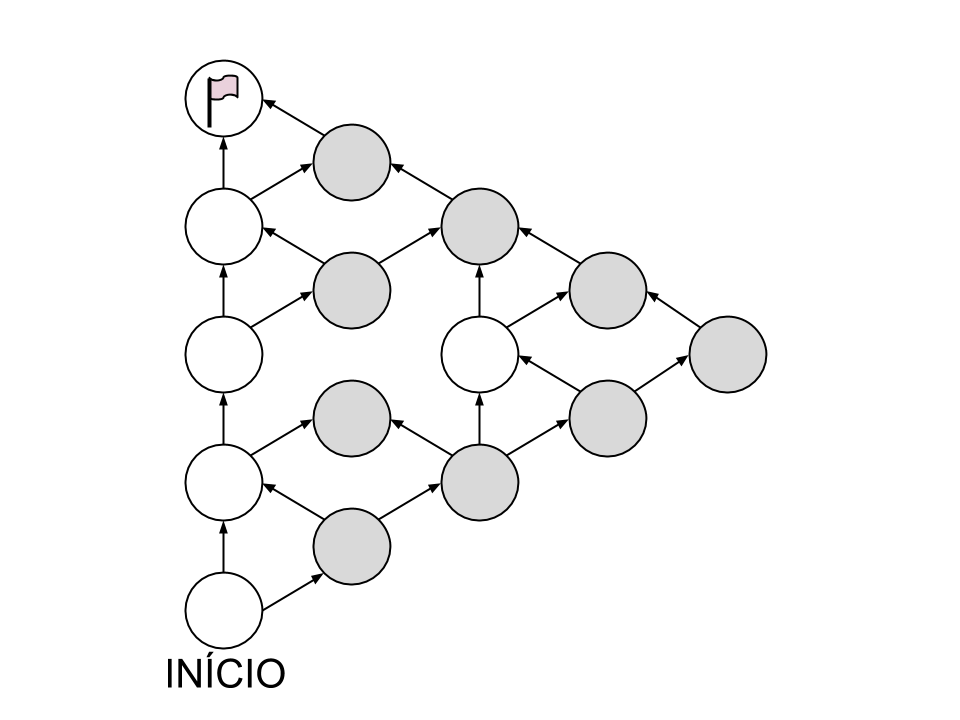
\includegraphics[width=8cm]{figures/tireworld.png}
  \caption{}
  \label{fig:tireworld}
\end{figure}


\subsubsection{Experimentos com o Domínio TireWorld}
\label{experimentosTireworld}


Rodamos os algoritmos com dez diferentes configurações de problemas para este domínio. Para cada diferente problema, o número de estados e as probabilidade das ações variaram.

%\begin{table}[H]

%TODO colar a tabela aqui
% nome do problema
% Quantidade de posições da grade
% quantidade de estados ruins para cada ação {norte, sul, leste, oeste}

\caption{}
\label{tab:tableTireworld}
\end{table}


\subsubsection{Resultados para o Domínio TireWorld}
\label{resultsTireworld}
A Figura \ref{fig:timeTW} exibe o tempo de execução de cada um dos algoritmos. Assim como no domínio Navigation, nos problemas do domínio Tireworld, o algoritmo $VI$ foi o que apresentou o pior desempenho em termos de tempo de convergência. Neste domínio, em todos os problemas, o $ILAO$ foi o que teve o menor tempo de convergência.

Nestes experimentos também usamos \textit{timeout} de um minuto para o algoritmo $RTDP$, o que pode explicar resultados muito acima dos demais algoritmos.

%Grafico para time - Tireworld
\begin{figure}[H]
\centering
\begin{tikzpicture}
  \begin{axis}[
%      only marks, 
      xtick=data, 
      xticklabels from table={plots/timeTW.dat}{Problema},
      xticklabel style={rotate=90},
      axis lines=left,
      xlabel={Problemas Tireworld},
      xlabel style={at={(0.5,-0.15)}},
      ylabel={Tempo de Execução em milissegundos},
      enlarge x limits={abs={0.0001*\pgfplotbarwidth}},
      legend style={at={(0.8,0.2)},anchor=north,legend columns=2},
      height=9cm, width=12cm,
      ymode=log]

      \addplot table [x expr=\coordindex,y=ILAO]{plots/timeTW.dat};
      \addplot table [x expr=\coordindex,y=RTDP]{plots/timeTW.dat};
      \addplot table [x expr=\coordindex,y=LRTDP]{plots/timeTW.dat};
      \addplot table [x expr=\coordindex,y=VI]{plots/timeTW.dat};

  \legend{ILAO, RTDP, LRTDP, VI}
  \end{axis}
\end{tikzpicture}
\caption{Tempo de Execução - Domínio Tireworld}
\label{fig:timeTW}
\end{figure}


A Figura \ref{fig:trialsTW} apresenta o número de \textit{trials} de cada um dos algoritmos ao longo de sua execução nas diferentes instâncias.

Neste domínio, o algortimo $LRTP$ executou mais \textit{trials} que o algoritmo $ILAO^*$, isso porque o algoritmo $ILAO$ atualiza mais estados a cada iteração. 


%Grafico Numero de trials - Tireworld
\begin{figure}[H]
\centering
\begin{tikzpicture}
  \begin{axis}[
      xtick=data, 
      xticklabels from table={plots/trialsTW.dat}{Problema},
      xticklabel style={rotate=90},
      axis lines=left,
      xlabel={Problemas Tireworld},
      xlabel style={at={(0.5,-0.15)}},
      ylabel={Número de \textit{Trials}},
      enlarge x limits={abs={0.0001*\pgfplotbarwidth}},
      legend style={at={(0.8,0.2)},anchor=north,legend columns=2},
      height=9cm, width=12cm, ymode=log]

      \addplot table [x expr=\coordindex,y=ILAO]{plots/trialsTW.dat};
      \addplot table [x expr=\coordindex,y=RTDP]{plots/trialsTW.dat};
      \addplot table [x expr=\coordindex,y=LRTDP]{plots/trialsTW.dat};
      \addplot table [x expr=\coordindex,y=VI]{plots/trialsTW.dat};
      %\addplot table [x expr=\coordindex,y=RTDP90]{plots/trialsTW.dat};

  \legend{ILAO, RTDP, LRTDP, VI}
  \end{axis}
\end{tikzpicture}
\caption{Número de \textit{Trials} - Domínio Tireworld}
\label{fig:trialsTW}
\end{figure}


A Figura \ref{fig:estadosTW} mostra a quantidade de estados visitados pelos algoritmos. 

Assim como no domínio Navigation, o algoritmo $VI$ visitou o maior número de estados em todos os problemas. Neste domínio, a diferença enter os estados visitados em cada um dos algoritmos foi muito pequena. Nos problemas pequenos (tw-01 e tw-02) o $RTDP$ foi o que visitou menos estados.

%TODO explicar figura
%Grafico Estados - Tireworld
\begin{figure}[H]
\centering
%\scriptsize
%\subfigure[ref2][Estados Visitados]{
\begin{tikzpicture}
  \begin{axis}[
      xtick=data, 
      xticklabels from table={plots/estadosTW.dat}{Problema},
      xticklabel style={rotate=90},
      axis lines=left,
      xlabel={Problemas Tireworld},
      xlabel style={at={(0.5,-0.15)}},
      ylabel={Número de estados Visitados},
      enlarge x limits={abs={0.0001*\pgfplotbarwidth}},
      legend style={at={(0.88,0.35)},anchor=north,legend columns=1},
      height=9cm, width=12cm,
      ymode=log
      ]

      \addplot table [x expr=\coordindex,y=vILAO]{plots/estadosTW.dat};
      \addplot table [x expr=\coordindex,y=vRTDP]{plots/estadosTW.dat};
      \addplot table [x expr=\coordindex,y=vLRTDP]{plots/estadosTW.dat};
      \addplot table [x expr=\coordindex,y=vVI]{plots/estadosTW.dat};

  \legend{ILAO, RTDP, LRTDP, VI}
  \end{axis}
\end{tikzpicture}
%}
%\subfigure[ref1][Número de estados visitados]{
%\begin{tabular}{|l|l|l|l|l|}
%\hline
%Prob. & ILAO & RTDP & LRTDP & VI  \\ \hline
%tw-01 & 15   & 12   & 16    & 24  \\ \hline
%tw-02 & 32   & 30   & 32    & 40  \\ \hline
%tw-03 & 52   & 50   & 54    & 60  \\ \hline
%tw-04 & 76   & 76   & 73    & 84  \\ \hline
%tw-05 & 104  & 104  & 105   & 112 \\ \hline
%tw-06 & 136  & 136  & 135   & 144 \\ \hline
%tw-07 & 172  & 172  & 169   & 180 \\ \hline
%tw-08 & 212  & 212  & 212   & 220 \\ \hline
%tw-09 & 256  & 256  & 254   & 264 \\ \hline
%tw-10 & 304  & 304  & 302   & 312 \\ \hline
%\end{tabular}
%}
\caption{Número de estados visitados- Domínio Tireworld}
\label{fig:estadosTW}
\end{figure}






%%%%%%%%%%%%%%%%%%%%%%%%%%%%%%%%%%%%%%%%%%%%%%%%%%%%%%

%TODO ler conclusao do Ignasi
\section{Conclusões}\label{conclusao}


Em geral, em nossos experimentos, o algoritmo $ILAO^*$ foi o que apresentou um melhor desempenho. Apenas em algumas instâncias menores, o $LRTDP$ teve uma performance melhor. 

Apesar de apresentar um tempo de convergência menor, a quantidade de estados vistados pelo $ILAO^*$ foi maior. Em relação ao estados relevantes, podemos afirmar que ambos algoritmos tentam reduzir o número de estados visitados, pois usam políticas gulosas. 

Um exemplo que ilustra isso, é o estado robot-at-x20-y04 (um estado irrelevante para os dois algoritmos). Nenhuma política ótima chega até ele. A principal diferença está em como tratar os possíveis efeitos não-determinísticos. O $LRTDP$ visita somente os estados mais prováveis, deixando muitas vezes de lado os estados que tem probabilidade baixa de serem alcançados, enquanto o algoritmo $ILAO^*$ não se limita em visitar apenas estados mais prováveis, mas todos os estados alcançáveis a partir de uma ação.



%%%%%%%%%%%%%%%%%%%%%%%%%%%%%%%%%%%%%%%%%%%%%%%%%%%%%%
\bibliographystyle{apalike}	% Tipo do formato da bibliografia
\bibliography{bibliografia}

\end{document}
